\chapter{Subsystem: Localization/Mapping} \label{chap:Localization}

% Need to talk about frames, sensors, kalman filtering scheme, hector_slam, results

\begin{figure}[H]
	\centerline{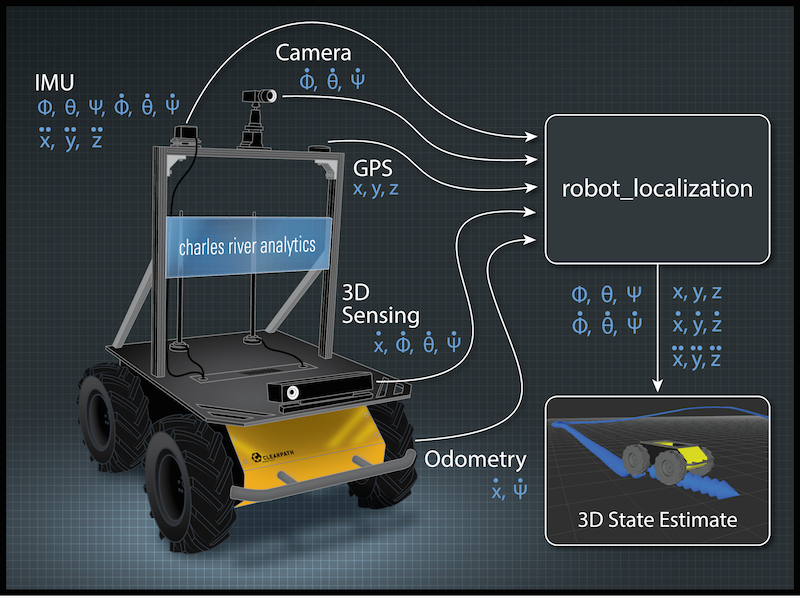
\includegraphics[angle=0,width=0.5\linewidth]{rl}}
	\caption[]{Localization Illustration \cite{clearpath}}
	\label{fig:robotlocalization}
\end{figure}

Localization is an important step for any autonomous or partially autonomous system hoping to navigate in the physical world. While autonomous driving does not fall within the scope of our project, localization is a necessary step for creating an accurate map of the environment. 

ROS provides a framework for developing localization systems and provides several cutting-edge algorithms for fusing sensor data into an accurate position estimate. For our vehicle we are combining the LIDAR, accelerometer, gyroscope, GPS, ans wheel sensor data using an Extended Kalman filter to generate an accurate position estimate. Using this position estimate, we will then build both 2D and 3D maps of the environment. 

We aim to have our system be able to determine the position of the Rover within 1 meter after traveling 100 meters and generate a map while traveling.

\section{Sensors}

%Tachometer,IMU,GPS,LIDAR

\begin{figure}[H]
	\centerline{\includegraphics[angle=0,width=0.5\linewidth,angle=90]{tach}}
	\caption[]{Hall Effect Tachometer}
	\label{fig:tach}
\end{figure}

The first sensor that incorporate into our localization scheme is the vehicle tachometer. The tachometer is an aftermarket sensor addition which senses the vehicle speed, which we consider to be a "body-frame forward" speed. The tachometer is actually two adjacent hall-effect sensors which sense the movement of the teeth on a gear fixed to the rear drive shaft. Through the use of dual hall-effect sensors, the sensor is able to output a quadrature signal from which both speed and direction can be extrapolated. The output of this sensor is fed to the 'Tachometer Arduino', which interprets the quadrature signal and feeds the resulting position and speed to the Vehicle Mega.

\begin{figure}[H]
	\centerline{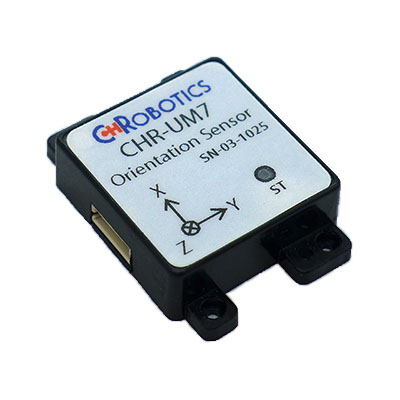
\includegraphics[angle=0,width=0.4\linewidth]{um7.jpg}}
	\caption[]{CH Robotics UM7 IMU}
	\label{fig:imu}
\end{figure}

The second source of data comes the Inertial Measurement Unit (IMU), which includes 3 sensors; a 3-axis accelerometer, a 3-axis gyro and a 3 axis-magnetometer. We chose the CH Robotics UM7 IMU to use on the vehicle because of it's relatively low price point, existing integration with ROS and it's active user base. Most modern IMU's have filtering on the device and in the case of the UM7, it outputs an orientation estimate (yaw,pitch,roll) as well as the raw sensor data. 

\begin{figure}[H]
\centering
\begin{subfigure}{.5\textwidth}
	\centering
	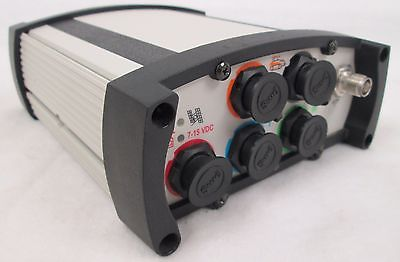
\includegraphics[width=.8\linewidth]{propak}
	\caption{GPS Receiver}
	\label{fig:sub1}
\end{subfigure}%
\begin{subfigure}{.5\textwidth}
	\centering
	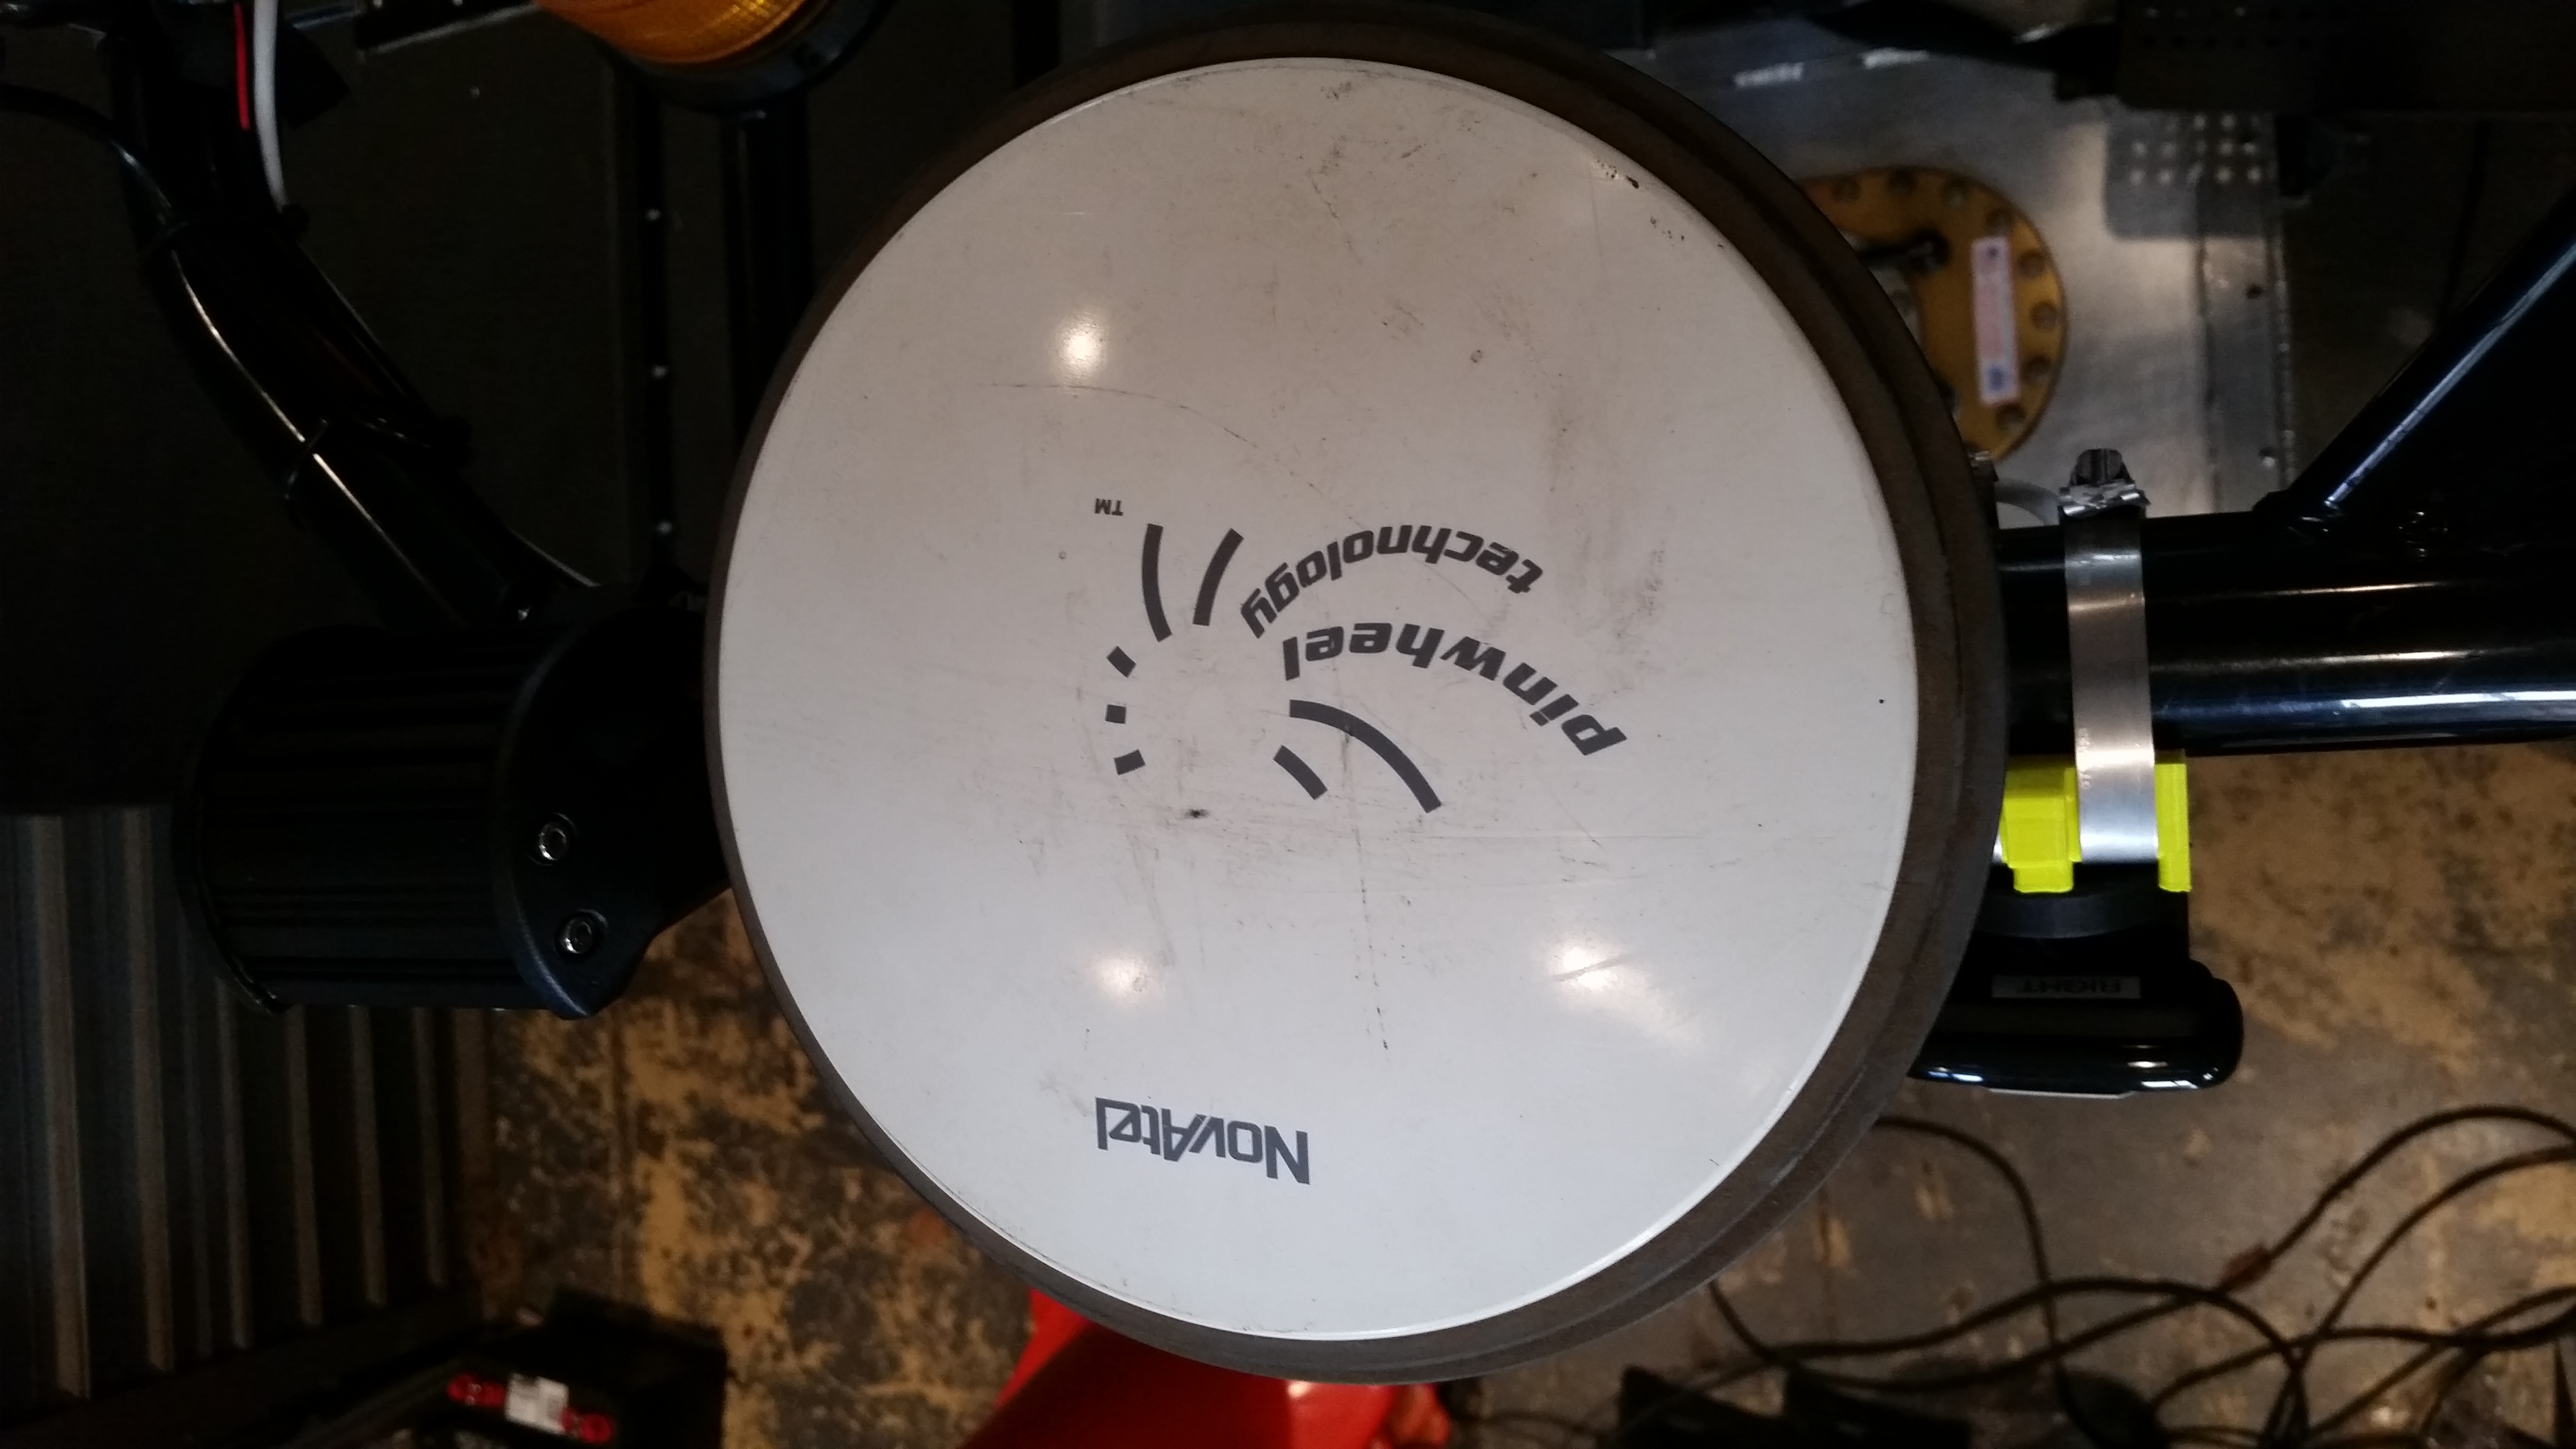
\includegraphics[width=.8\linewidth,angle=180]{GPSAntenna}
	\caption{GPS Antenna}
	\label{fig:sub2}
\end{subfigure}
\caption{Novatel ProPak-LB GPS System}
\label{fig:test}
\end{figure}

Next, the GPS unit, a Novatel Propak-LB, outputs position and velocity estimates in the form of standard NMEA strings. Preexisting ROS nodes (nmea\_serial\_driver) enable us to read in these NMEA strings over a usb-to-serial adapter and incorporate the GPS data into our state estimate. The GPS has the added benefit of performing it's own estimate of the covariance (a statistical measure of the estimate's certainty). The Kalman Filter utilizes the covariance to weigh the GPS more heavily when the GPS has more satellite's in view. Additionally, the GPS unit is capable of taking WAAS (Wide Area Augmentation System) GPS corrections into account. The WAAS system calculates and transmits corrections to increase the prevision of GPS receivers.

\begin{figure}[H]
	\centering
	\begin{subfigure}{.5\textwidth}
		\centering
		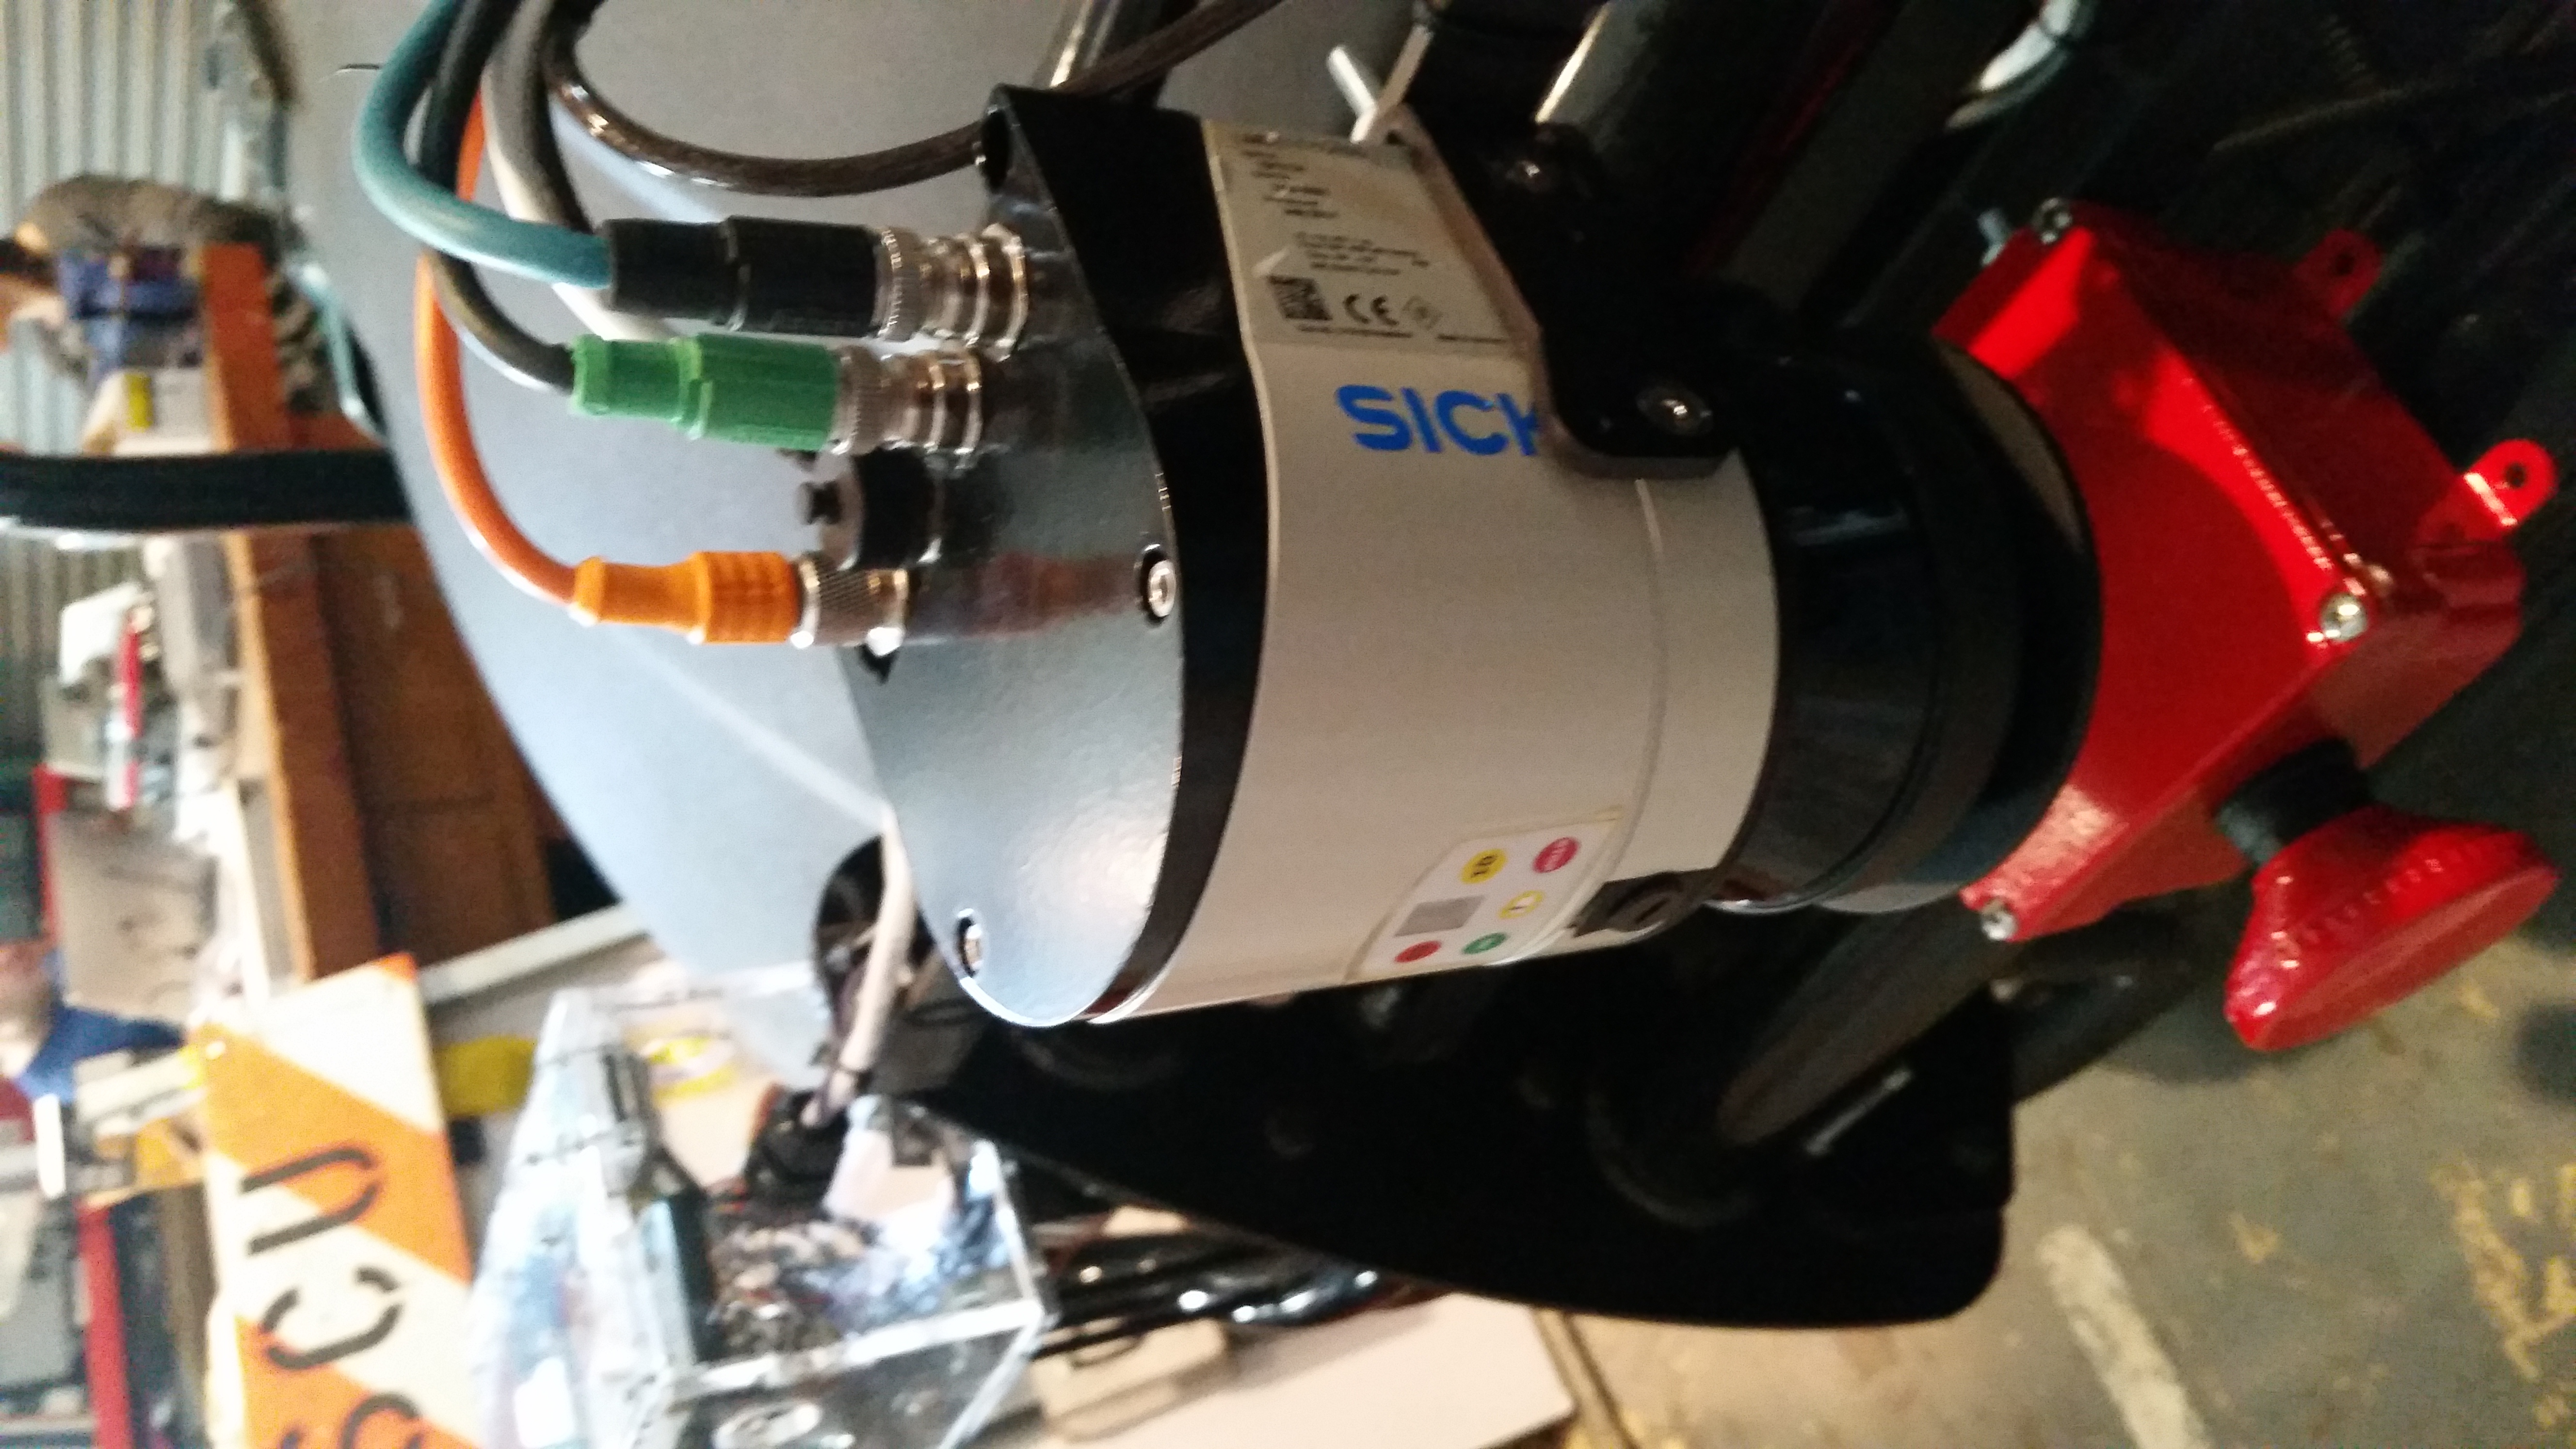
\includegraphics[width=.5\linewidth,angle=270]{LMS111_front}
		\caption{Front Mounted Static LIDAR}
		\label{fig:sub1}
	\end{subfigure}%
	\begin{subfigure}{.5\textwidth}
		\centering
		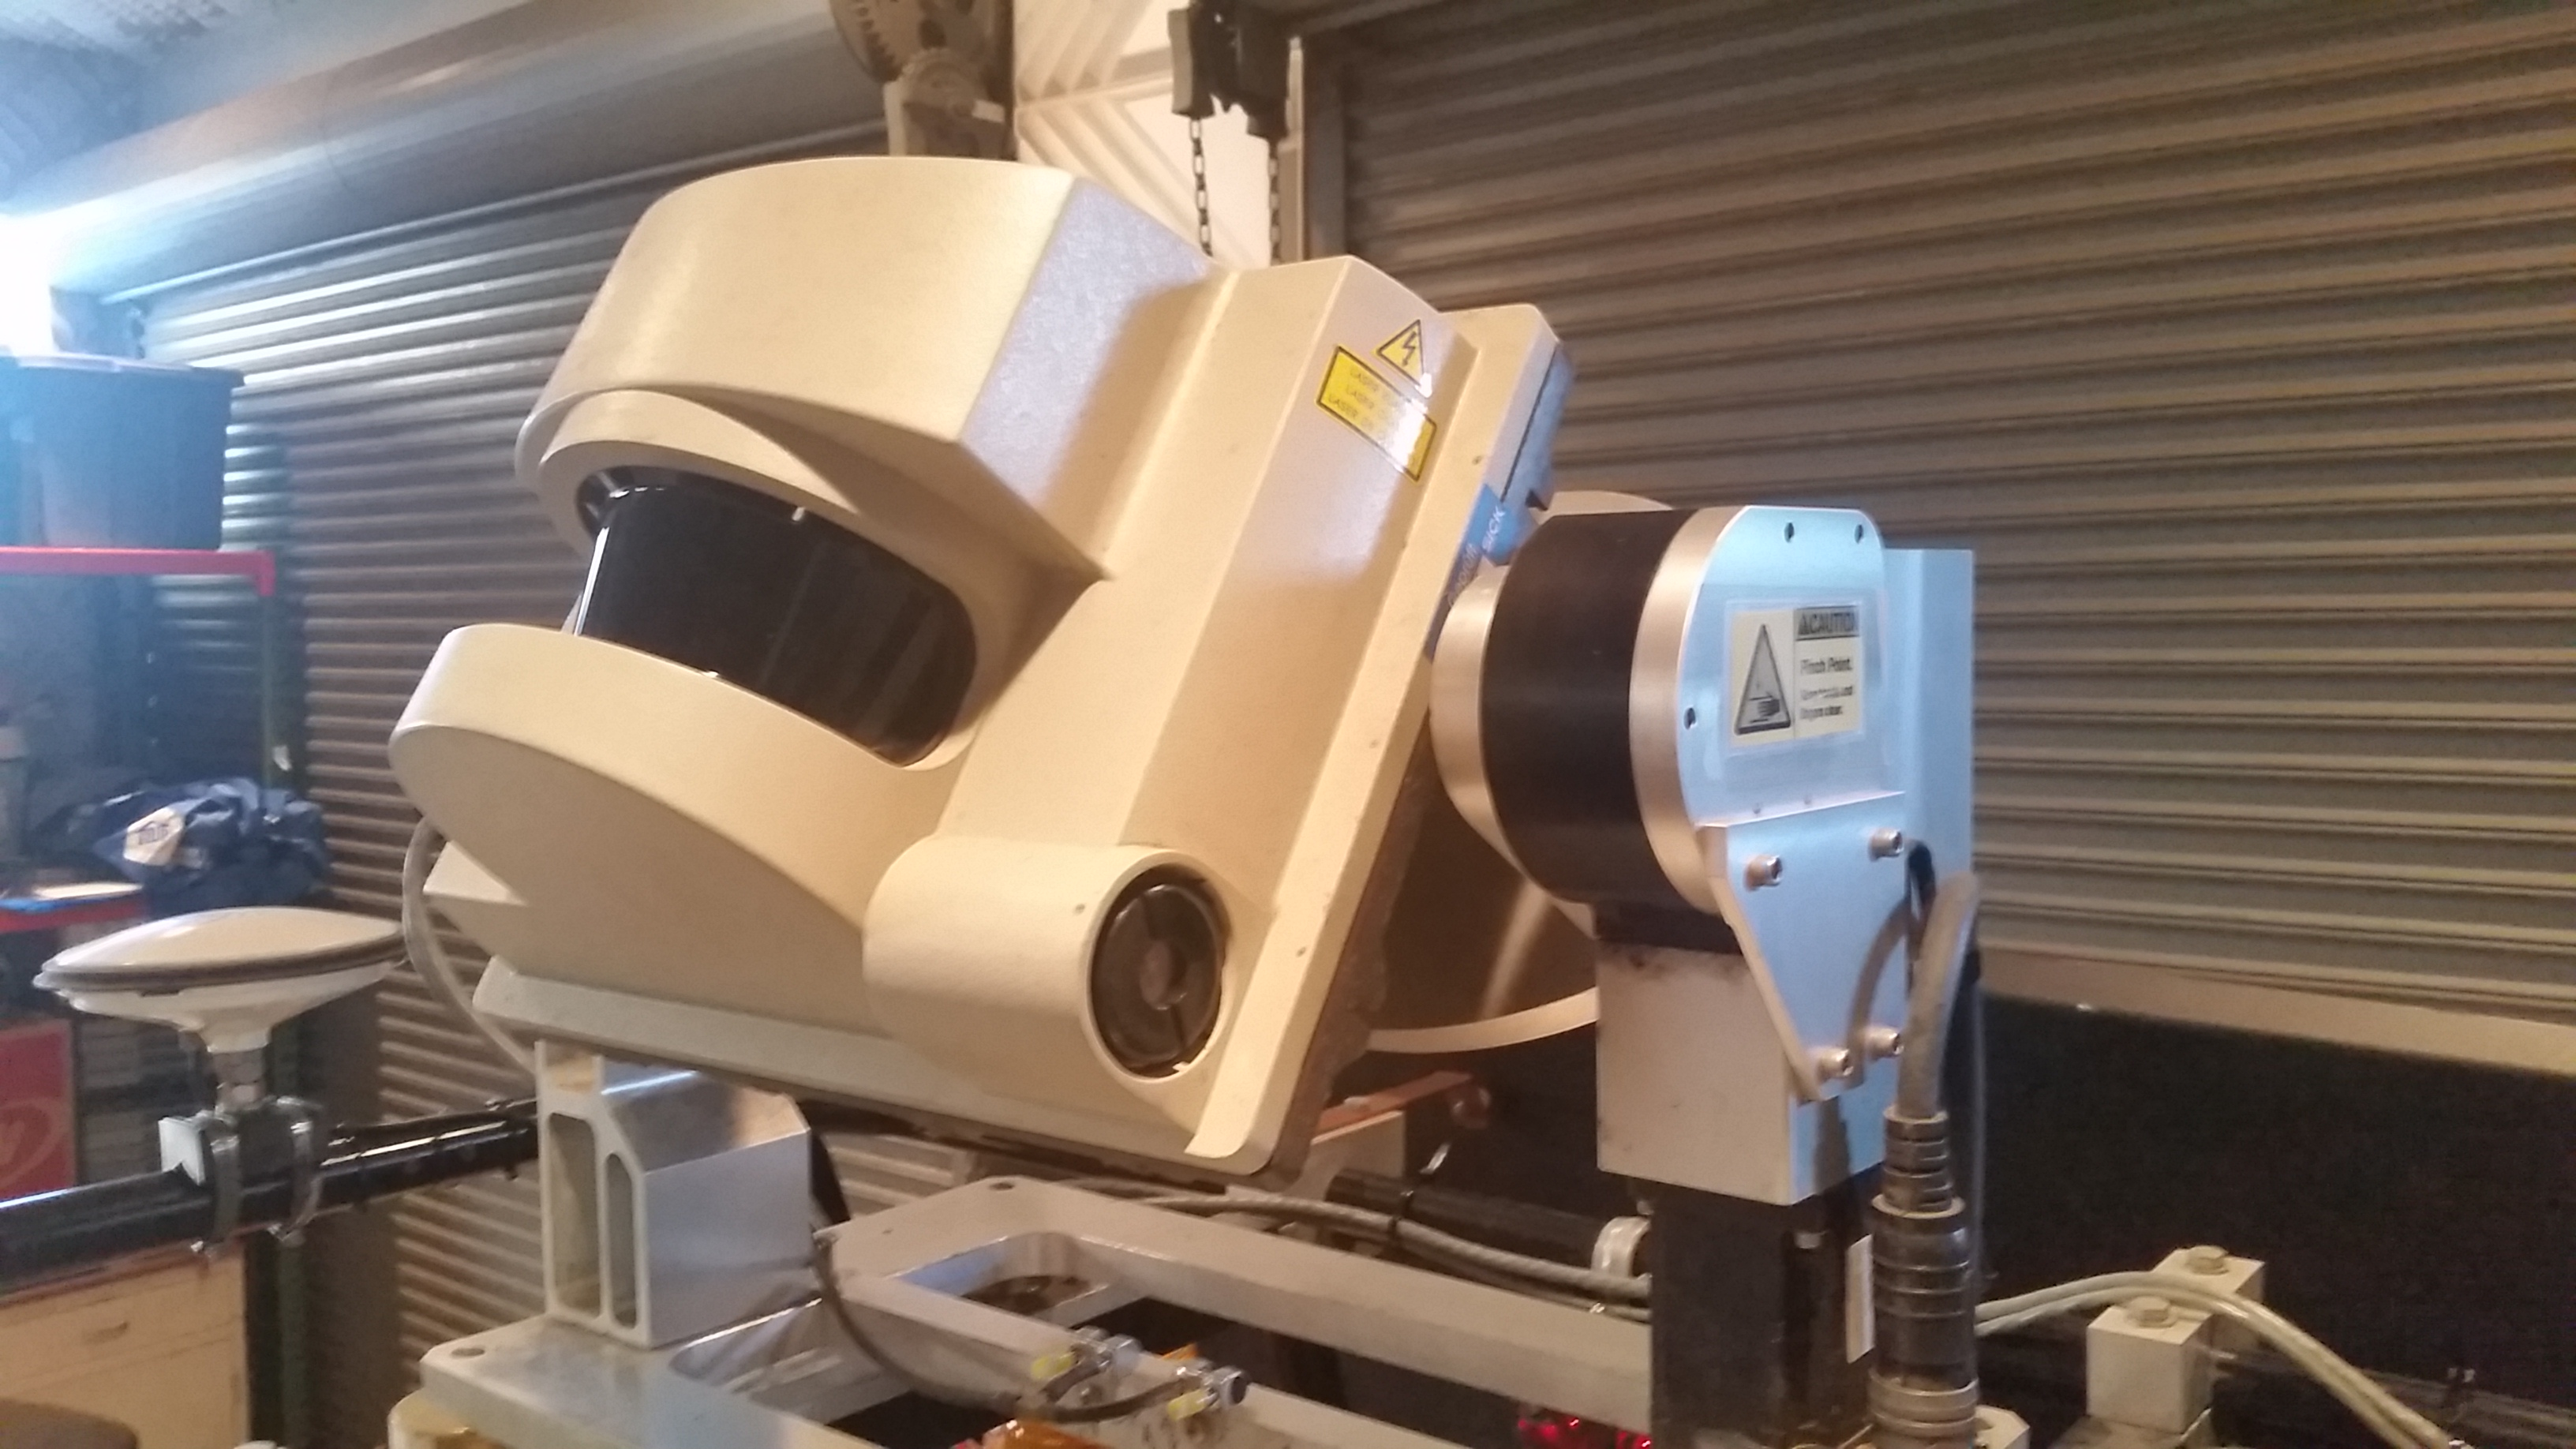
\includegraphics[width=.8\linewidth]{LMS221}
		\caption{Roll Cage Mounted Sweeping LIDAR}
		\label{fig:sub2}
	\end{subfigure}
	\caption{RSL Rover LIDAR Sensors}
	\label{fig:lidar}
\end{figure}

Finally, the rover has 2 lidar sensors available. A statically mounted unit on the front grill and a tilting unit on a gimbal mounted on top of the vehicle. For localization, we are using the unit mounted on the front of the vehicle, along with a ROS package called hector\_slam to produce an estimate for the robot's state. The SLAM (Simultaneous Localization and Mapping) process compares the current laser scan to a map or past data to estimate the movement of the vehicle. The SLAM process also provides us with a 2d map of the environment which can be saved and used for navigation at a later time.

\section{Coordinate Frames}

When developing a complex robotic system, keeping track reference frames for all of the different components of a robot is critical for determining the configuration of the robot in space. ROS has convenient functionality for not only defining coordinate frames, but also for calculating the transformations between them. 

Our first frame is the base\_link frame. By convention this is the highest level frame on the robot. For our purposes we chose to define the base\_link frame to be located at the centroid of the four rear tires with the X axis forward, Y axis left and Z axis up. The direction conventions are ROS standards, but the location of this was left to us. We chose this particular location, but based on the kinematics of the vehicle, the center of rotation of the vehicle should be around the centroid of the four rear wheels. 

The localization of the vehicle is performed in two stages, first taking into account only sensors which produce a continuous estimate of the robot state (ie. Tachometer, IMU) for use in the future autonomous driving and local path planning. The output of the localization defines a coordinate transform between \textbackslash base\_link and the \textbackslash odom frame.

The second state takes into account discontinuous sensor data (ie. GPS, SLAM) to produce a more accurate, but sometimes 'jumpy' position estimate. The advantage of using this frame is that when planning long-term navigation, this frame is not subject to the same drift that the odom frame is subject to. The second step in the localization process defines a transformation between the \textbackslash base\_link and the \textbackslash map frames.

\section{Kalman Filter}

We are using an implementation of an extended kalman filter for state estimation through the ROS robot\_localization package. This package takes input from an arbitarary number of sensors and produces an estimate of the robot's 15 dimensional state, [x,y,z,roll,pitch,yaw,vx,vy,vz,vroll,vpitch,vyaw,ax,ay,az]\cite{Moore2016}. 

As mentioned previously, the localization takes place in two steps. The first step defines the continuous estimate in the \textbackslash odom frame. For this step we only fuse the continuous estimates of the robot position, specifically the IMU and the tachometer. For each of these sensors, we only define a subset of their measured quantities to use. For example, with the IMU, we chose only to fuse the roll, pitch and yaw into the position estimate, excluding the raw angular rates, and accelerations, because they were already incorporated in the IMU's internal filters. Next, we chose to fuse the tachometer speed as a body-frame forward velocity for the rover. Using these two pieces of information, the IMU for the direction and the tachometer for the speed, we are able to get a rough position estimate for the rover. 

However, the as time increases, small bias errors or noise will accumulate to create a position estimate which is unusably incorrect. To compensate for this, we perform a second localization step which incorporates the GPS and SLAM functionality to provide absolute positioning relative to the environment. We fuse the same variables from the IMU and tachometers but then add the X,Y position from the GPS and X,Y velocities from the SLAM node. The \textbackslash map frame defined by this node has small discontinuous jumps, however its absolute position error does not grow continuously like the \textbackslash odom frame.

One of the features which was most frustrating to debug with the Kalman filter was the effects of the covariance matrix for each sensor. The covariance matrix represents the statistical confidence in the sensor data being reported. Some nodes, such as the GPS node and the SLAM node report an actual, dynamic covariance based on the performance of their algorithms. However, other sensors such as the IMU and Tachometer don't report covariance. In order for the kalman filter to output a valid estimate, we had to estimate these values. In order to do this, we viewed the stead state noise floor for each sensor and set the covariance such that it was slightly higher than this value. While not extremely accurate, this seemed to perform well and prevented the Kalman filter from propagating this noise into the position estimate.

\section{Hector SLAM}

%TODO: ADD HECTOR SLAM IMAGE

In order to generate a more accurate absolute position estimate than the GPS could provide, we turned to a SLAM (Simultaneous Localization And Mapping) solution. SLAM works by analyzing LIDAR data, comparing subsequent scans to determine a position and orientation estimate for the robot. In order to decrease the implementation time, we turned to several available ROS implementations of SLAM algorithms. The most common packages for SLAM are gmapping and hector\_slam. Both packages are 2D SLAM algorithms which compare planar laser scans to determine position. We chose to use hector\_slam due to the fact that an odometry input is not necessary.  

While we saw very good performance out of the SLAM system, there are several critical caveats which would make the currently available implementations not-ideal for our particular application. First, the SLAM algorithms have a fixed map of a fixed size. This essentially means that the area that the vehicle can navigate in is limited by the memory available on the laptop. An ideal solution and proven solution to this problem would be to have a rolling map, where only the map in the area surrounding the current rover is persisted. Secondly, through ROS we only had access to 2D SLAM implementations, which rely on the assumption that the environment is uniform in the vertical direction. While these implementations work very well in indoor environments with many vertical features, the outdoor environment, especially the natural outdoor environment has very few purely vertical features. In order to get better performance in an unstructured 3D environment, a 3D SLAM solution would be required

\section{3D Visualization}

%TODO: Pointcloud Photo

In addition to the 3D pointcloud which is visualized in the web UI, ROS's rviz utility was heavily utilized to visualize pointclouds and provide debugging information to both operators and developers. 

%TODO: Octomap Photo

Additionally, in post-processing we are able to feed the position estimates and LIDAR data into the Octomap ROS package. Octomap is a 3D occupancy grid implementation which allows the LIDAR not only to identify obstacles, but also clear obstacles from the map.

